%\vspace{-2cm}
\section{Introduction} 
\label{sec:intro}
In the subject of fluid dynamics, flow control can massively influence the performance of the flow around or inside an object. Designing a flow control method requires intricate understanding of flow behaviours such as dynamics and turbulence. Designing a proper flow control can be essential for maximising the efficiency of the system.


\subsection{Motivation}
\label{sec:motivation}
Climate change has been a driving factor for engineering design in the modern world \cite{Douglas2017}. The changes in climate pattern has proven to be detrimental to human and other living being. One of the causes of the climate change is the emission of energy generation process, such as carbon dioxide \cite{Met_Officend}. However, the need of creating more energy is indispensable as human population grows continuously, with energy requirement predicted to reach more than the triple of global energy requirement today \cite{IRENA2023}. This requires engineers to create a high performance solution with a consideration of efficiency in its operations. In aerospace sector, this approach is also used as the sector creates 2\% of the total global emission, which is the largest among other means of transportation \cite{Iea2023}. Generally in aerospace sector, high efficiency value can be reached by minimising drag, which generated from the viscous drag, as shown in Figure \ref{fig:B737}.
The viscous drag can be practically reduced in a controlled manner using flow control strategies, offers a solution for a sustainable aerospace future \cite{Abbas2017}.

\begin{figure}[ht]
    \centering
    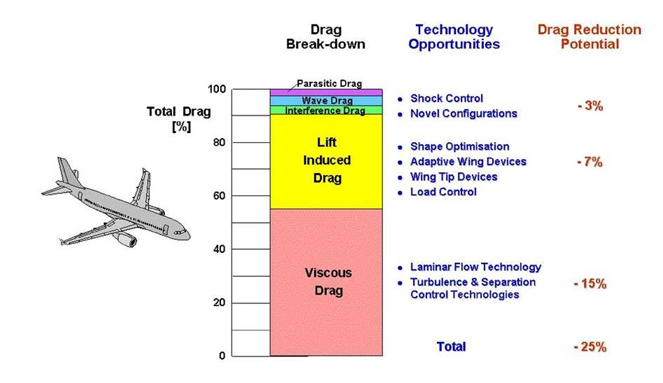
\includegraphics[width=0.75\linewidth]{Figures/B737Drag.png}
    \caption{Drag and Reduction Potential in a General Aircraft~\cite{Abbas2017}}
    \label{fig:B737}
\end{figure}


Fluid flow control has been a major topic in fluid dynamics. Fluid flow control strategies have been implemented in various areas, such as aerospace, wind energy sector, industrial process designs, and water management \cite{Airiau2016}. The development of flow control methods was born from the understanding of the presence of turbulence in a fluid flow. Turbulence in a moving flow can generally be denoted by the chaotic behaviour of the fluid \cite{Benzi2023}, typically in the form of eddies or vortices. The interaction of the flow with itself, along with the solid object nearby can produce drag, which reduces the flow velocity and its ability to transport its properties \cite{Bell1979}. In most systems, the drag can be detrimental as it can reduce the efficiency of the system. Because of that, flow control strategies are introduced to force the fluid to move in a regulated behaviour to decrease the drag produced in the system. 

Currently, multiple strategies and approaches towards an efficient flow control system are studied. One of recent studies \cite{Marusic2021} suggests that an active flow control strategy in the form of spanwise wall oscillations can generate a positive net power saving value for high Reynolds number regimes. With the finding, a pathway for an industrial-wide application of oscillating wall flow control can be opened and hence a further studies are needed.

In order to further expand the spanwise wall oscillation flow control strategy, understanding the turbulence in the flow is of utmost importance, especially in the near wall region. Turbulence is the chaotic nature of a fluid flow, caused by "a complex interplay of multiple flow patterns occurring simultaneously, making difficult to model and predict accurately" \cite{Alberti2023}. Therefore, intricate physics modelling is generally required to completely simulate the turbulence in the flow, which growingly expensive in terms of computational cost as the Reynolds number increases \cite{Chen2021}. In this paper, ensemble averaging is introduced as a solution for simulating intricate turbulence in a spanwise oscillating wall flow control analysis.



\subsection{Literature  Review}

\subsubsection{Physics of Wall Bounded Flow Turbulence}
\label{sec:litrev_oscwall}
Turbulence can be defined as the swirling motion that happened randomly in the fluid flow \cite{Sreenivasan1999}. Due to its randomness, turbulence phenomena can sometimes be too complicated and difficult to comprehend \cite{Hussain1986}. Therefore, most turbulence studies are focused on understanding the coherent structures, which are the regions with recognisable concentrated vorticity \cite{Fiedler1988}. As seen in Figure \ref{fig:hairpintamas}, there are common structures in the flow region near the wall that is identifiable. The most prominent structure is the hairpin vortex, which indicated by a raising arch head with two streamwise-oriented legs \cite{Wang2015}.
\pagebreak
\begin{figure}[ht]
    \centering
    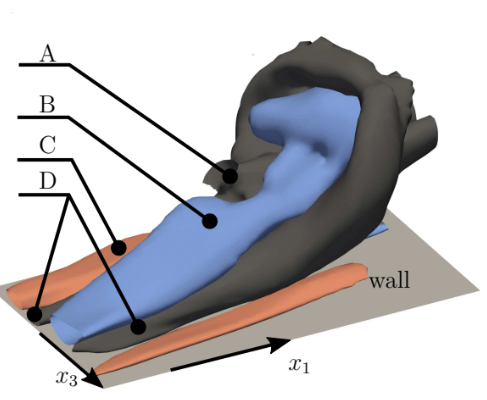
\includegraphics[width=0.5\linewidth]{Figures/Hairpin2.png}
    \caption{Near Wall Coherent Structures: A) Hairpin Vortex ; B) Low momentum region; C) high momentum region; D) counter-rotating quasi-streamwise vortices~\cite{Tamas2019}}
    \label{fig:hairpintamas}
\end{figure}

Several researches, such as the studies made by Wang \cite{Wang2015} and Alfonsi \cite{Alfonsi2006} explained how the hairpin vortices generated. First, the legs of the hairpin vortices, which consist of two quasi-streamline, counter-rotating vortices are interacted with each other. These vortices rises to the area with lower shear magnitudes, which decreases the vorticity magnitude. With the opposing rotational direction, the coalescence of two vortical structures are occurred and the hairpin vortices are generated. Inside the vortex, low momentum region is generated. Conversely, the high momentum region is generated outside the two counter-rotating vortices.

Other than the physical structures, the spectral analysis is also commonly conducted to understand the turbulence phenomena. Generally, spectral analysis involves analysing the turbulence through the wave energy distribution in the structures \cite{Fan2023}. In order to visualise the energy distribution, the Kolmogorov spectrum is used, as shown in the Figure \ref{fig:specturb}.

Based on Brennen \cite{Brennen2004}, there are 3 main regions in the spectrum. The first is the integral region, or commonly known as the energy containing range. This characterises the overall size of the largest eddies, which contains the energy in the flow. These large scale structures are responsible for transfering energy to the from the external forces to the smaller structures in the turbulent flow. The energy is then cascades to the smaller scales through the inertial region. The energy spectrum in this region follows a power law distribution:
\begin{equation}
    E(k) \propto k^{\frac53}
\end{equation}
Where k is wave number. Afterwards, the energy cascades to the smallest scales, which are in the Kolmogorov scales. In this scales, the viscosity dominates and the kinetic energy is transfered to heat energy.

\begin{figure}
    \centering
    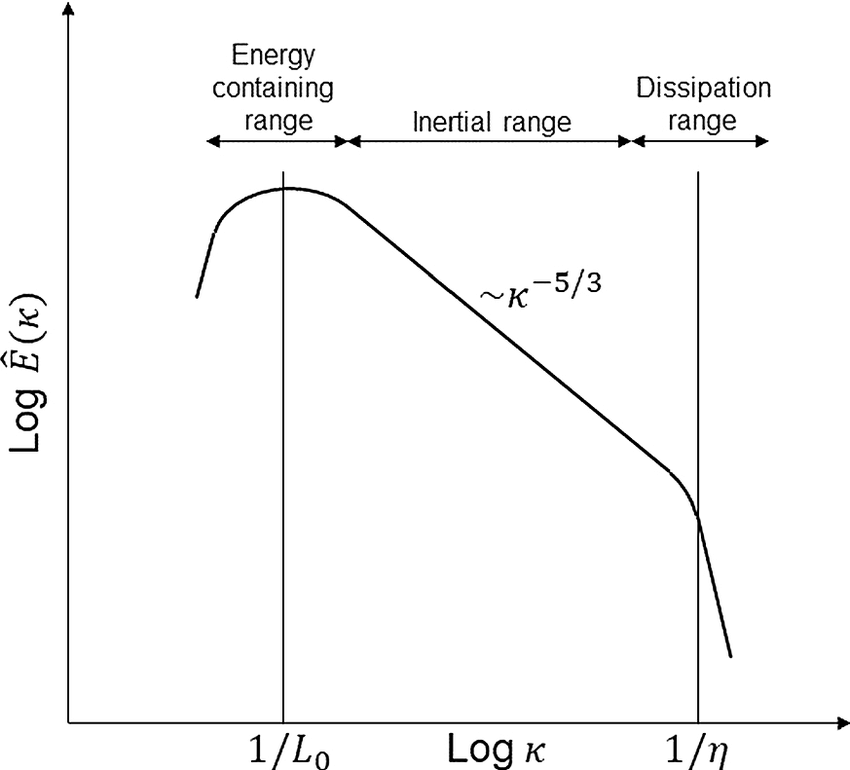
\includegraphics[width=0.65\linewidth]{Figures/KolmogorovSpectrum.png}
    \caption{Typical Energy Spectrum in a Flow ~\cite{kalmar-Nagy2019}}
    \label{fig:specturb}
\end{figure}

%Dont understand about hairpin, Add about spectral??



\subsubsection{Spanwise Oscillating Wall Flow Control}
\label{sec:litrev_oscwallfc}
Flow control can be defined as the method of altering the flow to a desired state or path \cite{Jahamiri2010}. Typically, there are two types of flow control methods, as stated by Ricco \cite{Ricco2021}. The first method is the passive flow control, which requires no actuation or movement in the system, thus no external energy required to control the fluid flow. The second method is the active flow control. Contrary to its passive counterpart, the active flow control requires energy to actuate a motion in a flow. 

Due to the certain energy consumption, most of the study regarding active flow control are circulated around the strategy to create a motion that has a positive net power saving. The same trend has been observed for spanwise oscillating wall method, which requires actuation to create an oscillation in the near wall region. The concepts and methods are documented in Table \ref{tab:studies_spowfc}. 

\pagebreak
\begin{landscape}
\begin{longtable}{@{}lllll@{}}
\caption{Experimental and Computational Studies of Spanwise Oscillating Wall Flow Control}
\label{tab:studies_spowfc}\\
\hline
\multicolumn{1}{c}{\textbf{References}} & \multicolumn{1}{c}{\textbf{Geometry}} & \multicolumn{1}{c}{\textbf{Methodology}} & \textbf{Reynolds Number} & \textbf{NPS$_{max}$ ($\%$)} \\ \hline
\endfirsthead
%
\endhead
%
\hline
\endfoot
%
\endlastfoot
%
Marusic et al. (2021) \cite{Marusic2021} & CF & \begin{tabular}[t]{@{}l@{}}Experimental: Hot-wire \\ anemometry\\ Computational: LES (dynamic \\ Smagorinsky)\end{tabular} & \begin{tabular}[t]{@{}l@{}}Re$_\tau$ = 6000\\ Re$_\tau$ = 12800\end{tabular} & \begin{tabular}[t]{@{}l@{}}$\sim$7\\ $\sim$2\end{tabular} \\
Gatti and Quadrio (2016) \cite{Gatti2016} & CF & Computational: DNS & \begin{tabular}[t]{@{}l@{}}Re$_\tau$ = 200\\ Re$_\tau$ = 1000\end{tabular} & \begin{tabular}[t]{@{}l@{}}5.3 $\pm$ 0.24\\ 3.9 $\pm$ 0.31\end{tabular} \\
Quadrio et al. \cite{Quadrio2009} & CF & Computational: DNS & Re = 4760 & 5 \\
Auteri et al. (2010) \cite{Auteri2010} & PF & \begin{tabular}[t]{@{}l@{}}Experimental, with DNS \\ comparison from \cite{Quadrio2009}\end{tabular} & Re = 4760 & 17 \\
Viotti et al. (2009) \cite{Viotti2009} & CF & Computational: DNS & Re$_\tau$ = 200 & 23 \\
Chandran et al. (2023) \cite{Chandran2023} & CF & \begin{tabular}[t]{@{}l@{}}Experimental: Drag Balance and \\ Hot Wire Anemometry\end{tabular} & 4500 $\leq$ Re$_\tau$ $\leq$ 150000 & \begin{tabular}[t]{@{}l@{}}ISA: -40\\ OSA: 5-10\end{tabular} \\
Deshpande et al. (2024) \cite{Deshpande2024} & CF & Computational: DNS & Re$_\tau$ $\approx$ 300 & Not reported \\
Nguyen et al. (2021) \cite{Nguyen2021} & CF (with square bar) & Computational: DNS & Re$_\tau$ = 218 & 0.8 \\
Ricco et al. (2012) \cite{Ricco2012} & CF (rough wall) & Computational: DNS & Re$_\tau$ = 200 & Not reported \\ \hline
\end{longtable}

\end{landscape}

The key trend from the results is the NPS value is dependent from various factors. It is apparent from the studies that the NPS value of of the flow control decreases as the Reynolds number increases \cite{Gatti2016} \cite{Quadrio2009}. Other than that, the net power saving also relies on the wave function applied. From the studies, it can be seen that the net power saving is positive when the wave function of the oscillating wall matches the large-scale eddies inside the flow \cite{Marusic2021}\cite{Chandran2023}.

Based on the table, a simple channel flow is the most common base case to test the effectivity of flow control. This is due to the simplicity of the flow modelling as the case only has two wall surface, generally placed on the top and the bottom of the domain. The domain surfaces on the side are assumed to be free surfaces \cite{Apsley2023}. To the boundary condition assignment, the effect of the wall in the flow will be easier to analyse without having to take account the wall perpendicular to the wall of interest.

\subsubsection{Turbulence Modelling}
\label{sec:litrev_turbmethod}
Solving turbulence is required in order to create a good model of a fluid flow. This is because turbulence is highly related to the transport of mass, energy, and other values in the flow \cite{Trench2023}. However, variety in the temporal and spatial scale of turbulence oftentimes requires high computational power \cite{Duraisamy2019}. To alleviate the excessive computational power, turbulence modelling is often used, generally in the form of Reynolds Averaged Navier Stokes (RANS) \cite{Sidik2020}. However, due to the nature of the modelling, some simplifications leads to information loss, especially regarding the energy cascade to the small scales \cite{bush2020}. Other approach that can be done is using the Large Eddy Simulation (LES). LES method solves large eddies directly, but uses modelling to solve the small eddies \cite{Zhiyin2015}. This way, high accuracy can be obtained for the large structures, while maintaining low computational expenses. However, similar to RANS modelling, inaccuracy can occur in small-scale turbulence \cite{Mason1994}.

In cases where the effect of small-scales turbulence are heavily considered, turbulence modelling is fully disregarded. This means that the Navier-Stokes equations are directly solved \cite{Moin1998}. These method of solving the fluid flow is termed Direct Numerical Simulation (DNS). Ideally, DNS should be performed with spatial resolution at least as large as the Kolmogorov scale, which the smallest eddies that can be produced by the flow \cite{Boschung2016}. However, the fine grid resolution will make the analysis prohibitively expensive. Therefore, lower resolution usually preferred to DNS methods. %How much?

\subsubsection{Generalised Richardson Extrapolation}
In a computational analysis, the domain settings may change the value of the results. The finer the settings is, the higher the quality of the results. However, finer results require high computational resources which limits the resolution of the model. To counter the problem. the Richardson extrapolation is usually used. Richardson extrapolation can be defined as the approximation of the ideal value of convergent value using \cite{roache2009verification}:
\begin{equation}
	f_{h=0} \stackrel{\sim}{=} \frac43 f_1 - \frac13 f_2
\end{equation}

However, most of the application of Richardson extrapolation are limited to the spatial convergence. The novel method of Richardson extrapolation includes temporal and domain size to determine the best resolution of a computational case. The combined resolution is expressed as:

\begin{equation}
	Normalised Resolution = \frac{\Delta x_e^{current}}{\Delta x_e^{finest}} \frac{\Delta t^{current}}{\Delta t^{finest}} \frac{t_{tot}^{finest}}{t_{tot}^{current}} \frac{L_e^{finest}}{L_e^{current}}
\end{equation}

\subsubsection{Sample Averaging}
To understand the overall trend of a numerical result, the result must be averaged. The averaging is normally done using two different method. First is time averaging, which is the more common practice in CFD analysis. Time averaging involves obtaining the flow properties such as velocities and pressure over a long period of time. After that, the flow value is averaged. This way, the fluctuations during a transient analysis can be avoided, thus making further calculations easier \cite{Kallio2015}. Because of this, the time-averaging method is popular in steady-state analysis \cite{Sodja2007}. However, the long period sampling time requires high computational resources, especially when high-fidelity approaches are used \cite{Makarashvili2016}.

The alternative method of sample averaging is using the ensemble averaging. By definition, ensemble averaging requires "averaging over numerous independent simulations"\cite{Tosi2021}. Ensemble averaging decreases the requirement of computational power, thus making the analysis more efficient, especially in high Reynolds number \cite{Makarashvili2016}. Currently, the method is not popular in fluid dynamics, but the method is commonly used in molecular dynamics, where time-averaging is very costly to perform \cite{Gordiz2015}.

In a practical sense, time and ensemble averaging have a possibility to have the correlating result to one and another. This commonly referred as ergodicity, a statistical property that exhibits that the system has the equal value of ensemble and time averaging \cite{Yamamoto2024}. Turbulent flow, as shown in recent study \cite{Galanti2004}, has known to be ergodic. Therefore, turbulent flow analysis can benefit from both methods without sacrificing the result generation.

\subsubsection{Xcompact3d}
\label{sec:litrev_ic3d}
The research mainly uses Xcompact3d to solve the fluid flow. Xcompact3d is a FORTRAN 90 based open-source software purposed to simulate incompressible fluid flows \cite{Bartholomew2020}. The software uses high order compact schemes \cite{Laizet2014}, which utilises shortened version of high order schemes. This way, the analysis will still satisfy the need of high resolution of high-order schemes, while maintaining simplicity of low-order schemes \cite{Laizet2009}, making the compact schemes a powerful and efficient tool to solve turbulence.

%Choice of the compact schemes
%Workflows

With the higher order schemes, the simulation can run high fidelity schemes to solve the viscous terms in the Navier-Stokes equation. The two models that are available to use in Incompact3d is Large Eddy Simulation (LES) and Direct Numerical Simulation (DNS) \cite{Laizet2014}. As the section \ref{sec:litrev_turbmethod} suggests, both methods are preferable when it comes to analysing turbulence in detail.

%%LES method --> simagorinsky
%%DNS Method???


\subsubsection{Knowledge Gap}
\label{sec:litrev_knowgap}
Current spanwise oscillating wall flow control research lacks a thorough analysis in high Reynolds number. To conduct flow control studies using CFD, researchers must analyse turbulence in great depth, usually using LES or DNS analysis. This leads to high computational expenses. The requirement of high computational power also increased with the increase of Reynolds number. Moreover, the studies conducted uses time--averaged approaches, further pushing the need of ensemble averaging approach as an alternative approach. With this study, future study can hopefully be conducted at a high Reynolds number region that could not be done before.


\subsection{Aim and Objectives}
\label{sec:Aim and objectives}
The aim of the study is to analyse the effectivity of ensemble averaging in numerical analysis of spanwise oscillating wall flow control.

With this aim, the objectives can be set as the steps to achieve the aim set. The objectives are set as follows:
\begin{itemize}[noitemsep]
    \item Generate a channel flow grid as a case for the study
    \item Generate a generalised Richardson extrapolation by changing the spatial and temporal resolution
    \item Conduct flow simulations of the channel flow with and without spanwise oscillating wall flow control using DNS
    \item Generate and compare the time and ensemble averaging results using post-processing methods

\end{itemize}



\subsection{Synopsis}
\label{sec:Sinopsis}
The thesis is arranged to be in a form as follows. Section \ref{sec:Methodology} provides the theoretical background and the methodology for the thesis. The governing equations, along with the supporting equations used in the numerical simulations are thoroughly explained. Moreover, the computational procedures, including geometry and mesh generations, simulations settings and post processing methods are introduced in this section.

Results obtained from the analysis is displayed in Section \ref{sec:Results & Discussion}. The discussion is then served as the rationale of the result. Several figures and tables are displayed as a summary for the result and an aid for understanding the phenomena behind the flow condition. Section \ref{sec:Conclusions & Recommendations} presents the conclusions of the current study and recommendations for future studies.
